\documentclass{../../class}

\title{4231 Homework 5}
\author{Eumin Hong (eh2890)}
\date{\today}

\begin{document}
\maketitle

\lhead{4231 Homework 5}
\rhead{Eumin Hong (eh2890)}

\tcbset{colback=blue!5, colframe=blue!75!black}

\section*{Problem 1}
\begin{tcolorbox}
    Exercise 22.2-8 on Page 602: Diameter of a tree. (Aim for a linear-time algorithm.)
\end{tcolorbox}

\subsection*{22.2-8}
The \textbf{\textit{diameter}} of a tree $T = (V, E)$ is defined as $\max_{u, v\in V} \sigma(u, v)$, that is, the largest of all shortest-path distances in the tree. Give an efficient algorithm to compute the diameter of a tree, and analyze the running time of your algorithm.

\newpage
\section*{Problem 2}
\begin{tcolorbox}
    Exercise 22.3-5 (c), 22.3-8, and 22.3-11 on Page 612. (For 22.3-11, you only need to give an example to show that the situation described here is possible. In both 22.3-8 and 22.3-11, the examples are very simple directed graphs.)
\end{tcolorbox}

\subsection*{22.3-5}
Show that edge $(u, v)$ is
\begin{itemize}
    \item[\textbf{\textit{c.}}] a cross edge if and only if $v.d < v.f < u.d < u.f$.
\end{itemize}

\subsection*{22.3-8}
Give a counterexample to the conjucture that if a directed graph $G$ contains a path from $u$ to $v$, and if $u.d < v.d$ in a depth-first search of $G$, then $v$ is a descendant of $u$ in the depth-first forest produced.

\subsection*{22.3-11}
Explain how a vertex $u$ of a directed graph can end up in a depth-first tree containing only $u$, even though $u$ has both incoming and outgoing edges in $G$.

\newpage
\section*{Problem 3}
\begin{tcolorbox}
    Exercise 22.4-2 on Page 614.
\end{tcolorbox}
\subsection*{22.4-2}
Give a linear-time algorithm that takes as input a directed acyclic graph $G = (V, E)$ and two vertices $s$ and $t$, and returns the number of simple paths from $s$ to $t$ in $G$. For example, the directed acyclic graph of Figure \ref{fig:dag} contains exactly four simple paths from vertex $p$ to vertex $v$: $pov$, $poryv$, $posryv$, and $psryv$. (Your algorithm needs only to count the simple paths, not list them.)
\begin{figure}[H]
    \centering
    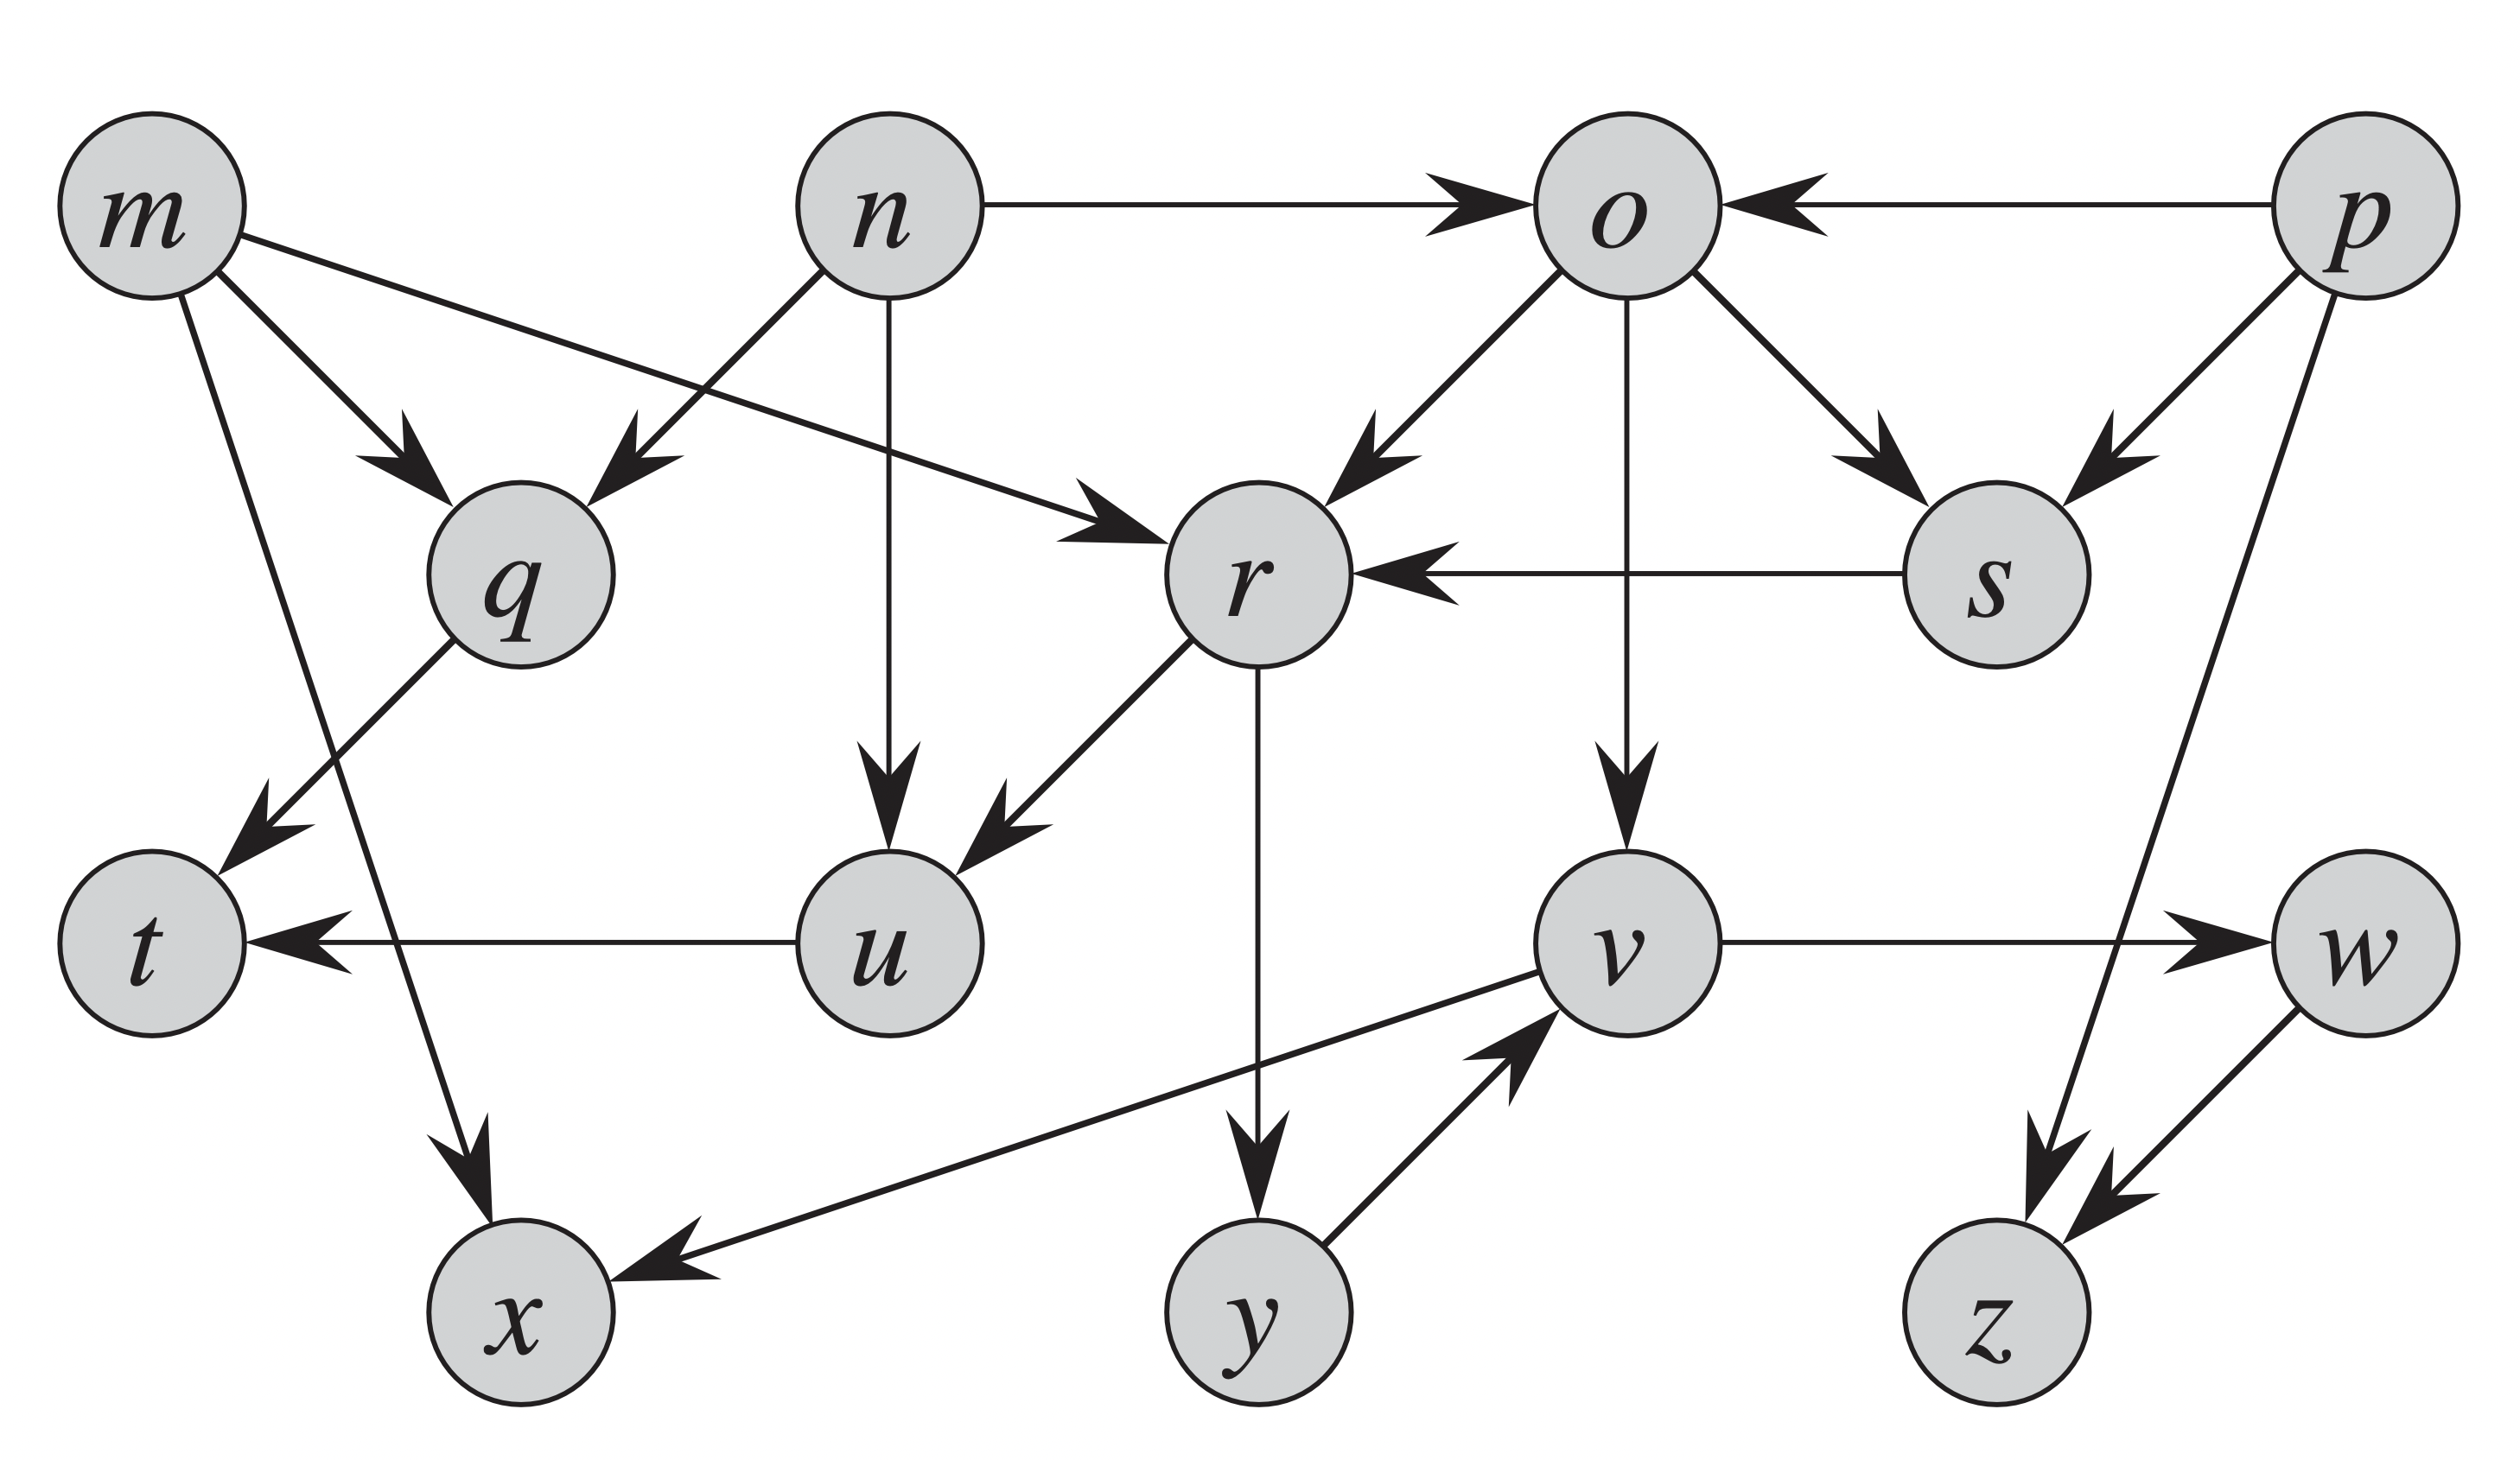
\includegraphics[width = 10cm]{img/dag.png}
    \caption{A dag for topological sorting.}
    \label{fig:dag}
\end{figure}

\newpage
\section*{Problem 4}
\begin{tcolorbox}
    Exercise 22.5-7 on Page 621.
\end{tcolorbox}
\subsection*{22.5-7}
A directed graph $G = (V, E)$ is \textbf{\textit{semiconnected}} if, for all pairs of vertices $u, v\in V$, we have $u \leadsto v$ or $v \leadsto u$. Give an efficient algorithm to determine whether or not $G$ is semiconnected. Prove that your algorithm is correct, and analyze its running time.

\newpage
\section*{Problem 5}
\begin{tcolorbox}
    Exercise 23.1-3 and 23.1-8 on Page 629.
\end{tcolorbox}
\subsection*{23.1-3}
Show that if an edge $(u, v)$ is contained in some minimum spanning tree, then it is a light edge crossing some cut of the graph.

\subsection*{23.1-8}
Let $T$ be a minimum spanning tree of a graph $G$, and let $L$ be the sorted list of the edge weights of $T$. Show that for any other minimum spanning tree $T'$ of $G$, the list $L$ is also the sorted list of edge weights of $T'$.

\end{document}
